\section{Cholesky 分解：把正能量写成平方和}
\label{sec:03-Linear-Algebra/06-Symmetric-and-Positive-Definite-Matrices/03}

一段 Gaussian process 回归的代码跑到第 40 轮超参数搜索时抛出异常：矩阵不是正定的。核矩阵是你亲手构造的，理论上一定半正定，怎么会失败？

这行报错来自 Cholesky 分解。它之所以能当成正定性的检测器，是因为它本身就是正定性的构造性证明：分解走得通，矩阵就正定；走不通，一定有某个方向的能量不为正。搞清楚这件事，报错信息就从``程序坏了''变成了一条关于模型或数据的诊断。

上一节把正定性等价地写成``二次型是一组线性表达式的平方和，且不留零方向''。特征分解给出的是正交的那一组，要先解一个特征值问题。Cholesky 换一组不正交但三角的表达式：

\[
A=LL^{\trans},\qquad L\ \text{下三角，对角元为正}.
\]

代进去立刻得到

\[
x^{\trans}Ax=x^{\trans}LL^{\trans}x=\norm{L^{\trans}x}^2 .
\]

\(L\) 对角元为正故可逆，\(L^{\trans}x=0\) 只在 \(x=0\) 时发生，所以这个方向的推理是一行的事：存在这样的 \(L\)，就有 \(A\succ0\)。真正需要论证的是反方向。

\subsection{存在性证明就是算法本身}

设 \(A\succ0\)，按第一行第一列分块：

\[
A=\begin{pmatrix}a&b^{\trans}\\b&C\end{pmatrix}.
\]

取 \(x=e_1\) 得 \(a=e_1^{\trans}Ae_1>0\)，所以 \(\sqrt a\) 有意义。这是分解的第一列能写下来的全部理由，把它记成 \(\ell_{11}=\sqrt a\)，\(\ell_{21:n}=b/\sqrt a\)。剩下要处理的是 \(n-1\) 维的矩阵

\[
S=C-\frac{bb^{\trans}}{a},
\]

即 \(A\) 关于第一个变量的 Schur 补。整个证明只剩一句话要说：\(S\) 仍然对称正定，于是同样的动作可以在低一维上重做，\(n\) 步之后收工。

\(S\) 正定的理由不必硬算。把 \(x\) 写成 \((x_1,u)\)，二次型是

\[
q(x)=a\,x_1^2+2x_1\,b^{\trans}u+u^{\trans}Cu .
\]

固定 \(u\ne0\)，关于 \(x_1\) 这是一条开口向上的抛物线，在 \(x_1=-b^{\trans}u/a\) 处取最小，最小值恰是 \(u^{\trans}Su\)。而那个取到最小的 \(x\) 不是零向量（它的后 \(n-1\) 个分量就是 \(u\)），由 \(A\succ0\) 得 \(q>0\)，故 \(u^{\trans}Su>0\)。

这段推理值得多看一眼：Schur 补就是``把第一个变量按最优方式消掉之后剩下的二次型''。消元、配方、Cholesky 递推、条件高斯分布的协方差，四件看起来不同的事共用这一个对象。至于展开成逐元素的递推公式是什么样子，那是把上面这段递归写成两重循环的结果，任何数值库里都有现成实现，手推一遍的收益不高。

\begin{proposition}
实对称矩阵 \(A\) 正定，当且仅当存在对角元为正的下三角矩阵 \(L\) 使 \(A=LL^{\trans}\)；此时 \(L\) 唯一。
\end{proposition}

唯一性来自逐列的构造没有留下任何选择：每一步的对角元被开方钉死（取正根），非对角元被除法钉死。顺带说明，\(L\) 与 \hyperref[sec:03-Linear-Algebra/01-Linear-Systems-and-Matrices/03]{``逆矩阵与 LU 分解：撤销变换并复用消元''}里的消元是同一件事——对称正定矩阵做 Gauss 消元永远不需要换行，主元全为正，写成 \(A=LDL^{\trans}\)（\(L\) 单位下三角，\(D\) 正对角）后把 \(D^{1/2}\) 吸收进 \(L\) 即得 Cholesky。省下的一半存储和一半运算，来自对称性：上三角部分不必单独存，它是下三角的转置。

\subsection{它把球形噪声塑成指定形状}

\(A=LL^{\trans}\) 最常被用到的地方也许不是解方程，而是采样。若 \(z\sim\mathcal N(0,I)\)，令

\[
x=\mu+Lz,
\]

则 \(\E x=\mu\)，且 \(\Cov(x)=L\,\Cov(z)\,L^{\trans}=LL^{\trans}=A\)。一堆各向同性的独立标准正态数，经 \(L\) 一乘就长出了指定的相关结构。

\begin{center}
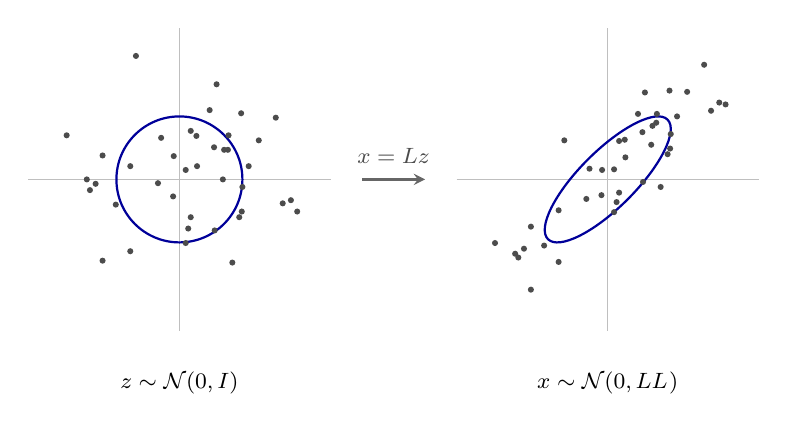
\begin{tikzpicture}[x=0.8cm,y=0.8cm,font=\small,>=stealth]
  \draw[black!25] (-2.4,0) -- (2.4,0);
  \draw[black!25] (0,-2.4) -- (0,2.4);
  \draw[blue!60!black,thick] (0,0) circle (1);
  \foreach \a/\b in {-1.22/0.38, 0.99/-0.51, -1.33/-0.07, 0.48/1.10, -1.22/-1.29,
    0.71/0.47, 1.53/0.98, -0.10/-0.27, -0.78/-1.14, 0.10/0.15, -0.34/-0.06, 0.27/0.69,
    1.10/0.21, -1.79/0.70, -1.42/-0.17, -1.47/0.00, -0.78/0.21, 0.84/-1.32, -0.29/0.66,
    -0.09/0.37, 0.10/-1.01, 0.56/-0.81, 1.87/-0.51, 0.69/0.00, 0.95/-0.60, 1.00/-0.12,
    1.26/0.62, 0.14/-0.78, 0.77/0.47, 1.64/-0.38, 0.55/0.51, 0.28/0.21, 0.18/-0.60,
    -1.01/-0.40, 0.59/1.51, 0.98/1.05, 0.78/0.70, 0.18/0.77, 1.77/-0.33, -0.69/1.96}
    \fill[black!70] (\a,\b) circle (1.1pt);
  \node[below,font=\footnotesize] at (0,-2.9) {\(z\sim\mathcal N(0,I)\)};
  \draw[->,thick,black!60] (2.9,0) -- (3.9,0);
  \node[above,black!70,font=\footnotesize] at (3.4,0.1) {\(x=Lz\)};
  \begin{scope}[shift={(6.8,0)}]
    \draw[black!25] (-2.4,0) -- (2.4,0);
    \draw[black!25] (0,-2.4) -- (0,2.4);
    \begin{scope}[rotate=45]
      \draw[blue!60!black,thick] (0,0) ellipse (1.342 and 0.447);
    \end{scope}
    \foreach \a/\b in {-1.22/-0.75, 0.99/0.49, -1.33/-1.10, 0.48/1.04, -1.22/-1.75,
      0.71/0.85, 1.53/1.82, -0.10/-0.25, -0.78/-1.31, 0.10/0.16, -0.34/-0.31, 0.27/0.63,
      1.10/1.00, -1.79/-1.01, -1.42/-1.24, -1.47/-1.18, -0.78/-0.49, 0.84/-0.12,
      -0.29/0.17, -0.09/0.15, 0.10/-0.52, 0.56/-0.04, 1.87/1.19, 0.69/0.55, 0.95/0.40,
      1.00/0.72, 1.26/1.39, 0.14/-0.36, 0.77/0.90, 1.64/1.09, 0.55/0.75, 0.28/0.35,
      0.18/-0.21, -1.01/-1.05, 0.59/1.38, 0.98/1.41, 0.78/1.04, 0.18/0.61, 1.77/1.22,
      -0.69/0.62}
      \fill[black!70] (\a,\b) circle (1.1pt);
    \node[below,font=\footnotesize] at (0,-2.9) {\(x\sim\mathcal N(0,LL^{\trans})\)};
  \end{scope}
\end{tikzpicture}

\emph{同一批 40 个标准正态样本，左边落在圆形云里，右边是每个点乘上 \(L=\bigl(\begin{smallmatrix}1&0\\0.8&0.6\end{smallmatrix}\bigr)\) 之后的位置。圆被拉成沿 \((1,1)^{\trans}\) 方向伸长的椭圆，点云跟着倾斜，两个坐标从此相关。蓝线是相同``\(1\sigma\)''水平的等高线，它的两条主轴由 \(LL^{\trans}\) 的特征向量给出，半轴长是特征值的平方根。}
\end{center}

反过来乘 \(L^{-1}\) 就是白化：\(L^{-1}(x-\mu)\) 把相关的高斯向量拉回标准正态。这两个方向一起用，就是从``模型里的协方差''到``可以喂进标准正态发生器的坐标''之间的往返票，重参数化技巧、卡尔曼滤波的平方根形式、扩散模型里的噪声调度，用的都是这张票。

\subsection{一次分解，两笔账同时结清}

多元高斯的对数密度里有两样东西要算：二次型 \((x-\mu)^{\trans}A^{-1}(x-\mu)\) 和 \(\log\det A\)。Cholesky 一次分解把两样都交出来。

二次型那边不必求逆。解三角方程 \(Lw=x-\mu\)，则 \(w^{\trans}w\) 就是所要的值，因为 \(A^{-1}=L^{-\trans}L^{-1}\)。行列式那边更直接：\(\det A=(\prod_i\ell_{ii})^2\)，于是

\[
\log\det A=2\sum_i\log\ell_{ii},
\]

全程是正数取对数再求和，不会像连乘那样溢出。GP 的边缘似然、EM 里的高斯 M 步、变分推断的 KL 项都要反复算这两样，Cholesky 是那里的默认工具，\hyperref[sec:13-Machine-Learning/09-Kernel-Methods-and-Gaussian-Processes/05]{``Gaussian process 把核变成函数先验''}会把整条计算链走一遍。

解线性系统同理：\(Ax=b\) 拆成 \(Ly=b\) 与 \(L^{\trans}x=y\) 两次三角回代。相比一般 LU，运算量与存储都约减半，而且不需要选主元——主元恒正这件事已经由正定性保证。对称正定系统的首选直接解法就是它。

有一处需要克制。最小二乘的正规方程 \(A^{\trans}A\hat\beta=A^{\trans}b\) 系数矩阵正定，用 Cholesky 解很省事，但显式形成 \(A^{\trans}A\) 会把条件数平方：\(A\) 的条件数 \(10^{6}\) 到了 \(A^{\trans}A\) 就是 \(10^{12}\)，双精度下有效数字几乎耗尽。数据病态时该走 QR 或 SVD，见 \hyperref[sec:03-Linear-Algebra/07-SVD-and-Data-Applications/02]{``伪逆与病态问题''}。快不等于稳。

\subsection{分解失败时它在告诉你什么}

回到开头那行报错。半正定矩阵允许零特征值，Cholesky 走到某一步会遇到零主元；数值上更常见的是遇到一个理论上应为零的微小负数，开方直接失败。所以失败信号真正在说的是``这个矩阵在数值意义下没有严格正的能量''，至于原因，通常是三类之一。

第一类是模型确实没保证正定。用一个自定义的相似度函数当核，若它不满足 Mercer 条件，核矩阵本来就可能有负特征值，这时该改的是核而不是数值细节。第二类是数据让矩阵退化：两个样本点重合、两列特征完全共线、样本量小于维度，理论上的正定被数据打到了半正定的边界上。第三类是舍入与病态：矩阵数学上正定，但条件数上到 \(10^{12}\)，最小特征值在浮点噪声里淹没了。

实践中的常用补救是加一个小的对角项 \(A+\varepsilon I\)，把所有特征值抬高 \(\varepsilon\)。这个动作在数值上永远有效，但它不是免费的：\(\varepsilon\) 在 GP 里就是观测噪声方差，在岭回归里就是正则强度，在协方差估计里就是往先验收缩。既然它改变了模型，就该像超参数那样报告和调节，而不是当作让程序跑通的一行补丁。若非要保留原矩阵，还可以换带主元的 Cholesky、\(LDL^{\trans}\) 或直接做特征分解，它们能处理半正定并顺手给出秩。

值得留下的是这个习惯：Cholesky 失败是一次免费的假设检查。矩阵按理该正定却分解不了，说明``按理''那一步的某个前提没有兑现，先去看前提，再去看数值。

正定性到这里已经有了判据、有了构造、有了实现。剩下没有回答的是最直观的那个问题：\(x^{\trans}Ax=c\) 这条曲面究竟长什么样，中心在哪，主轴朝哪个方向多长。下一节把谱分解和平移配方一起用上，让形状自己显出来。
